	
	The aim of this thesis is to explore the relatively new field of machine
	learning on graphs/networks. In particular, this thesis will focus on graph 
	machine learning applications for the purpose of gaining customer insights. 
	Graph machine learning is a current frontier in machine learning and has vast
	applications in many areas as recently shown by the success of AlphaFold
	\citep{senior2020improved}. AlphaFold made a breakthrough for predicting
	protein structures where they made use of the observation that a folded
	protein can be considered as a spatial graph \citep{AlphaFoldTeam2020}. In
	addition, there is a vast range of applications for graphs in the fields of 
	natural science, social science and many more as shown by the excellent 
	overview given by \cite{zhou2020graph}. In principle, graphs are useful 
	whenever one wants to consider the interactions between observations. Graph
	machine learning has therefore become a promising field as it allows for
	the consideration of standard observational data as well as any prevalent
	interactions or relationships between the observations. The field of graph 
	machine learning focuses on the developing methods which can exploit this 
	richer information for various tasks such as (customer-) classification. To
	provide a better understanding on how graphs in general as well as graph
	machine learning are relevant to business \& economics related fields such
	as gaining customer insights, some motivating examples are provided in the
	following section.

	\section{Relevance to Economics}

	\noindent From a business \& economics perspective, graphs are particularly
	interesting if one wants to for instance model the interactions between
	institutions. An example for this is a study published by
	\cite{schweitzer2009economic} which created a graph showing the 
	interdependencies or interactions of international banks as a network shown 
	in figure \ref{fig:bank_network}. This is a useful representation of 
	such interdependencies and provides important information for making the
	banking system more robust and resilient. 

	\begin{figure}[h]
		\centering
		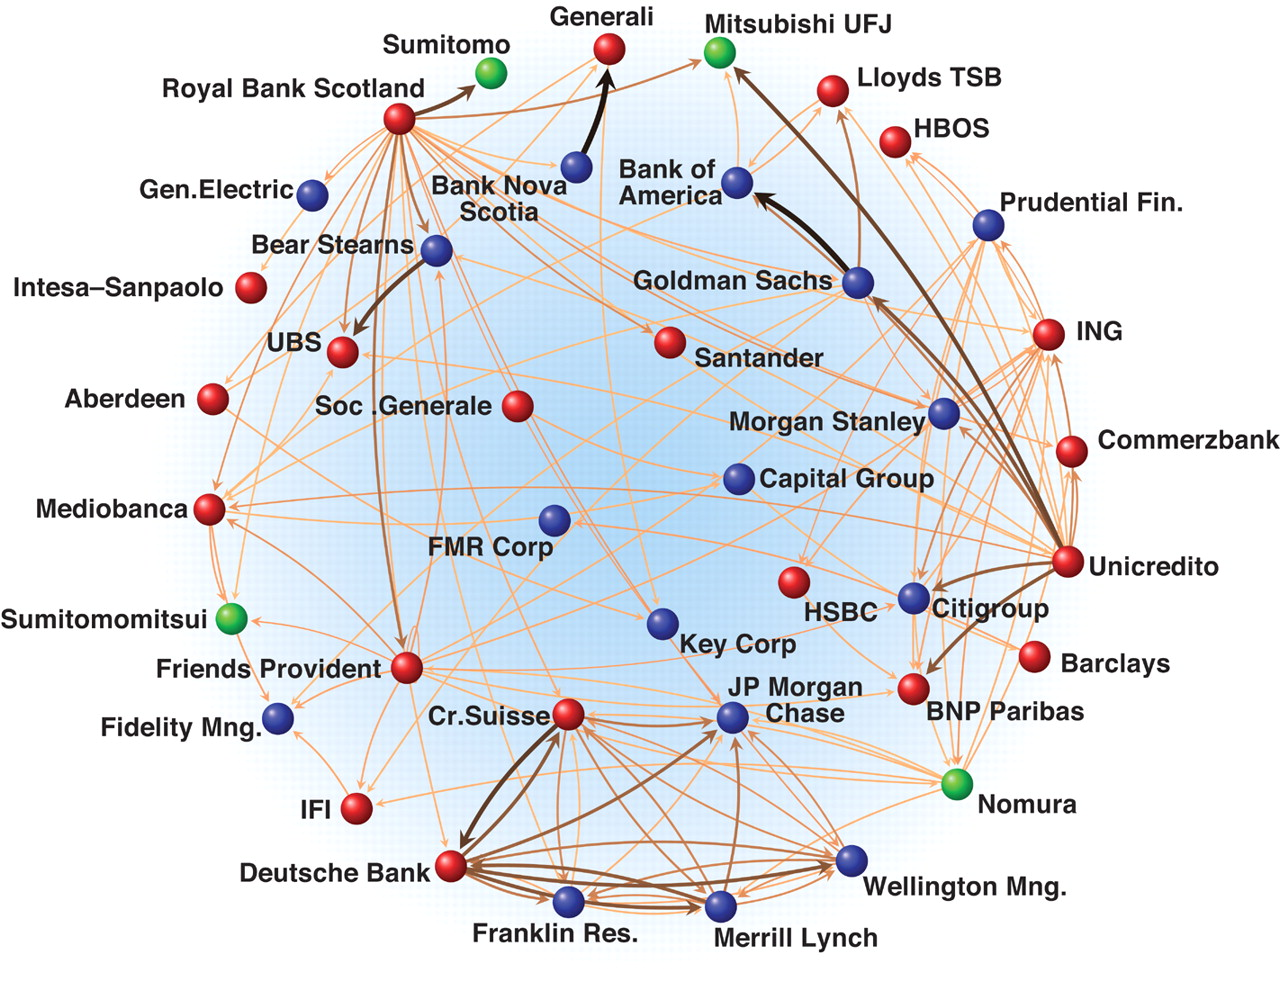
\includegraphics[width=0.5\textwidth]{bank_network.jpg}
		\caption{Bank Network}
		\cite[p. 424]{schweitzer2009economic}
		\label{fig:bank_network}
	\end{figure} 

	\noindent Another interesting application of graphs for business \& 
	economics are social interactions. While there are many different
	interesting applications where social interactions are of interest,
	the focus for this thesis is placed on gaining customer insights for the 
	purpose of improving products \& services as well as marketing. Indeed, 
	this is one of the main areas where social networks such as Facebook or 
	search providers like Google make their revenue by providing consumer
	insights or selling targeted advertising \citep{Facebook2021,Alphabet2021}. 
	Both Facebook and Google have the advantage, that their businesses 
	naturally capture relational or more generally network data which can be 
	represented as graphs. Most researchers or companies however do not have 
	access to such data. Companies for instance may have access to large 
	amounts of customer data, however they typically would not have access to 
	relational information (e.g. which client is connected with which other 
	clients). The same is true for researchers, where social scientists often 
	collect data via anonymous surveys which make the collection of network
	data basically impossible. In most cases this means, that companies or
	researchers can only generate- or have access to data which does not
	contain relational information such as social interactions or connections. 
	It is important to highlight, that there is a lot of social network data 
	available online. This network data however typically only contains the 
	network structure/connections. The feature data such as demographic data or
	topic specific variables of interest of the people present in the network 
	is however typically not provided. Without any feature data, graphs provide 
	rather limited information and in many cases are not useful for tasks such
	as providing customer insights. This is an issue in terms of data access 
	and is a frustrating reality which also affects this thesis. It however also
	motivated the research question which will be presented in the following 
	section.
	
	\section{Research Topic}
	\label{section:research_topics}

	\noindent The difficult access to graph data which included feature
	information, motivated the search for alternatives. A review of the
	literature revealed, that a form of synthetic graph generation could
	provide a solution to the data access problem. Classic graph generation
	procedures include the famous Erdös-Rényi graphs \citep{erdos1959random},
	the small-world model by \cite{watts1998collective}, the well-known model
	by \cite{barabasi1999emergence} and more recently Kronecker Graphs by
	\cite{leskovec2010kronecker}. These models are all very instructive
	regarding the graph generation process and for understanding graph
	properties. These networks however all have the short-coming, that they do 
	not allow for assigning feature data to the network. It became clear, that 
	one would have to find or develop a method which makes use of feature data 
	for the graph generation process. Fortunately, such a method was developed 
	by \cite{kim2012multiplicative} which introduced Multiplicative Attribute 
	Graphs (MAG). This model uses feature data which is referred to as 
	attribute data by the authors to generate graphs and appears to yield the 
	desired result of graph with feature data. This model and its 
	specifications will be introduced in detail in the theory section. \\

	\noindent More recently, researchers have focused their attention to
	generative graph models. These models create graphs with features using
	real graphs as a training input. Examples for such models are Graph
	Recurrent Neural Networks \citep{you2018graphrnn} and deep generative graph
	models \citep{li2018learning}. These are very fascinating models which can
	be used to recreated or scale graph data. For the purpose of this thesis,
	these methods were not purposeful, as it requires existing graph data to be
	present. For this thesis this unfortunately not the case. Nevertheless,
	this is an interesting current topic for graph generation. \\ 

	\noindent The access problem to graph data therefore might be resolved
	using the MAG method. This method is interesting as most researchers or
	companies have access to large amounts of feature data such as customer 
	databases or feature data which can be created using well-known methods
	like survey. It could therefore be of interest to generate a semi-synthetic 
	graph with the MAG method using more available non-graph data. 
	Semi-synthetic refers to the fact, that the synthetic graph is generated 
	using real collected feature data. Therefore it is referred to as
	semi-synthetic and differs to the fully synthetic methods previously outlined.
	The hope is, that relational information generated in the graph would
	provide useful additional information for machine learning task such as
	gaining customer insight. The aim of the thesis is therefore to investigate
	to what extent semi-synthetic graphs are useful for graph based machine
	learning techniques. Of course, semi-synthetic graphs cannot replace real
	graphs and graph machine learning on semi-synthetic graphs is unlikely to
	perform as well as it would on real graphs. It is however possible, that
	graph machine learning on semi-synthetic graphs is competitive, if not
	superior to machine learning methods which are not graph based and can only
	consider feature data. In order to assess the viability of this approach,
	the results using graph machine learning will be compared to standard
	machine learning approaches. To provide a better overview, a high level 
	overview of machine learning is provided in the following section. To close
	this section, the research question is presented formally as follows: \\

	\noindent\textbf{Research Question:}\\

	\textbf{To what extent are semi-synthetic graphs based on real 
				feature data useful for machine learning?}

	\section{Overview Machine Learning}

	This section will provide a high-level overview of machine learning and
	will specify the type of machine learning task used in this thesis. To
	start, it is important to correctly categorize machine learning. There are
	many related big topics such as data science, big data or artificial
	intelligence and it is often not clear what exactly is meant. A good
	graphical overview was generated by the Frauenhofer Institut and is shown
	in figure \ref{fig:ml_overview}.

	\begin{figure}[h]
		\centering
		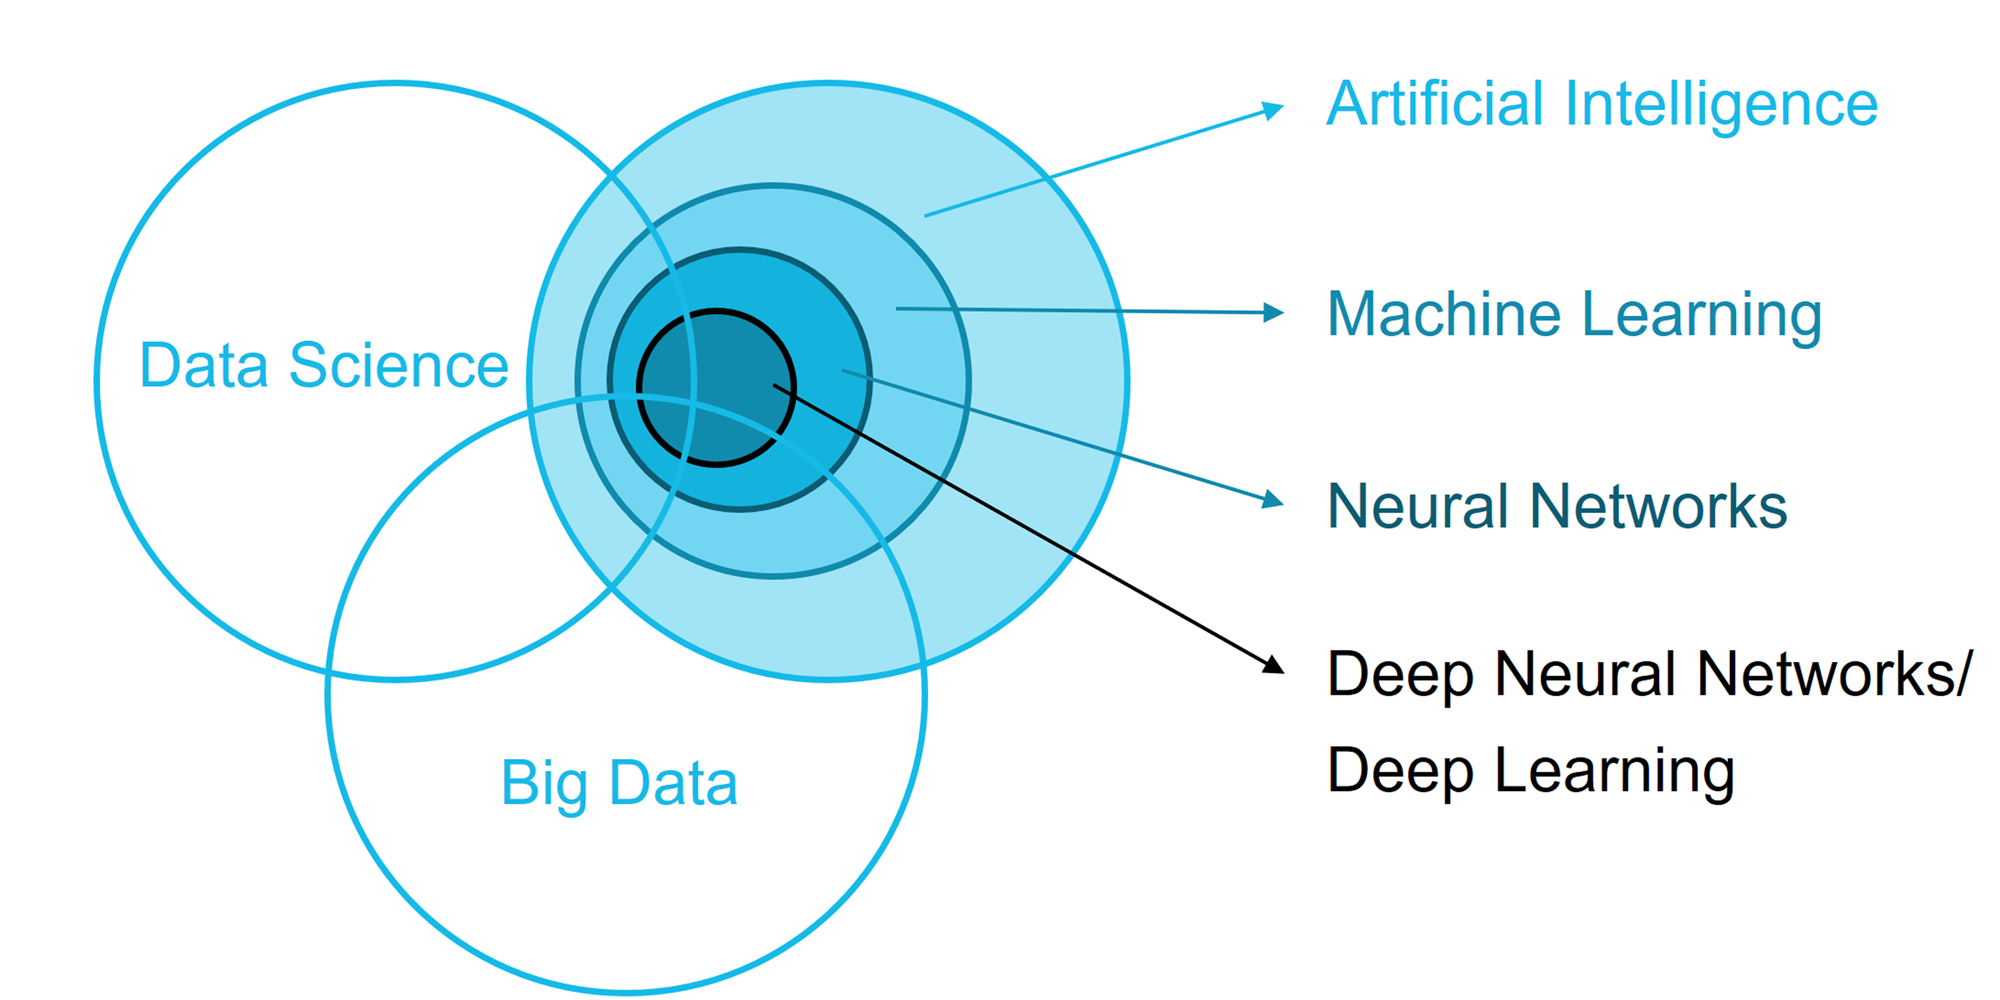
\includegraphics[width=0.7\textwidth]{overview_datascience.png}
		\caption{Overview Machine Learning}
		\cite{Frauenhofer2021}
		\label{fig:ml_overview}
	\end{figure} 

	\noindent Figure \ref{fig:ml_overview} shows well, how these different
	terms are related with each other. Machine learning in particular, is
	mostly ascribed to the domain of artificial intelligence, it however also
	shares its domain with data science and big data. It is thus at the
	intersection of these three main domains. Machine learning techniques such
	as neural networks and deep neural networks are specific methods within
	machine learning and are often referred to separately due to their
	popularity. In this thesis, differentiating between machine learning and
	neural networks is not necessary as all considered machine learning methods
	will be used for the same task. Machine learning can be applied for various
	tasks and is again best presented visually in figure \ref{fig:ml_tasks}.

	\begin{figure}[h]
		\centering
		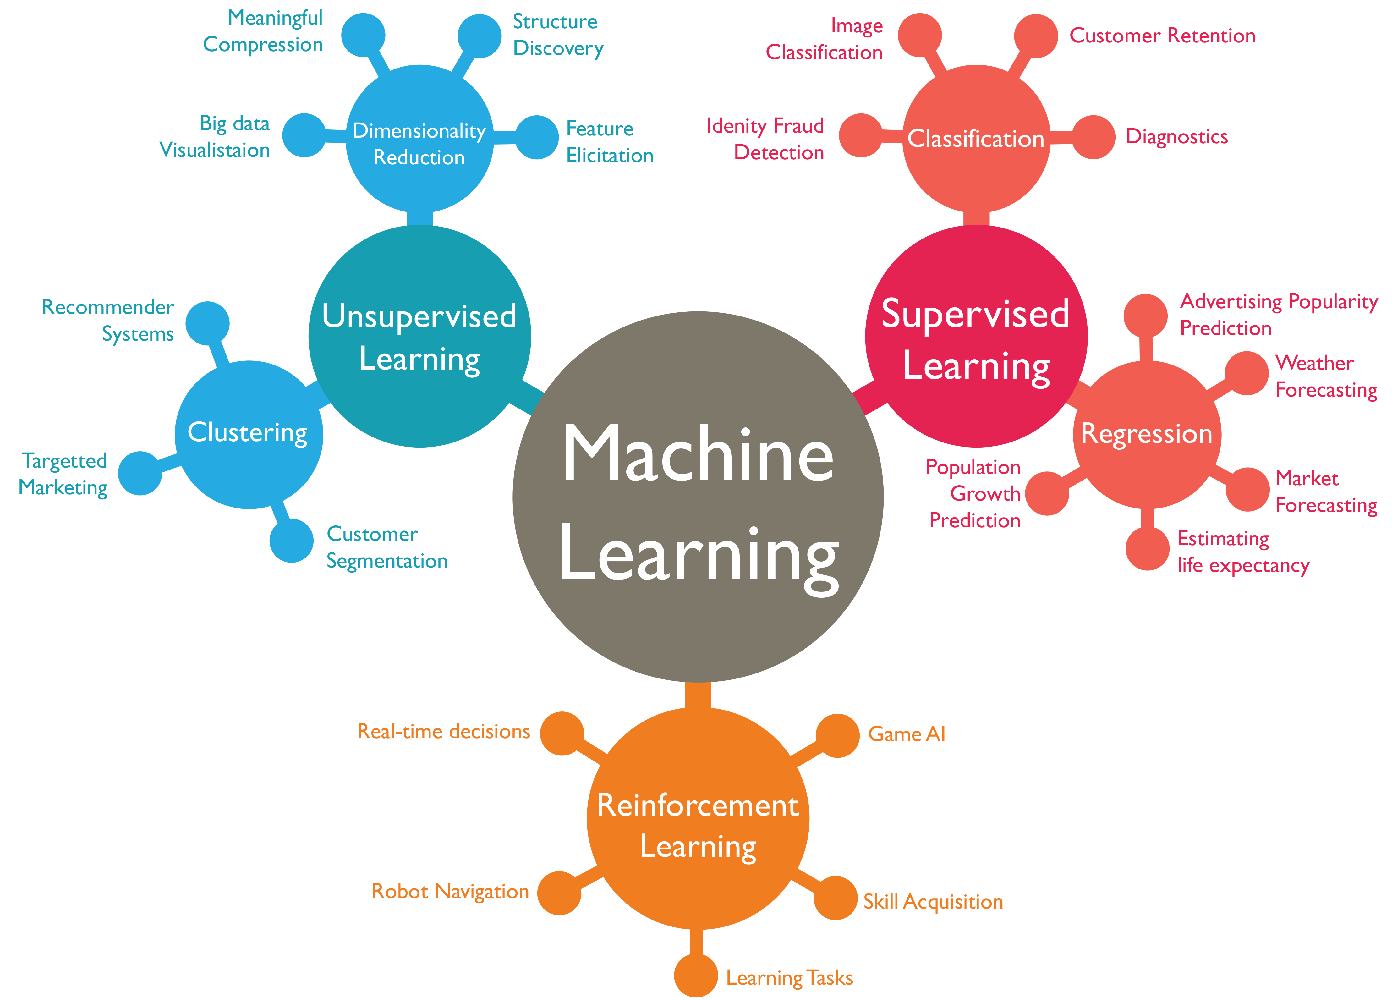
\includegraphics[width=0.8\textwidth]{ml_tasks.png}
		\caption{Overview Machine Learning Tasks}
		\cite{Artisan2020}
		\label{fig:ml_tasks}
	\end{figure} 

	\noindent It is shown in figure \ref{fig:ml_tasks} that the main tasks for
	machine learning involve classification, regression, reinforcement
	learning, clustering and dimensionality reduction. This thesis will focus
	on classification tasks. This task was chosen given the available data for
	this thesis and because it allows for a nice comparison of different
	methods. Well known standard machine learning methods for classification tasks
	include logistic regression \citep{cramer2002origins}, naive bayes
	\citep{zhang2004bayes}, support vector machines
	\citep{platt1999probabilistic}, random forest classifiers
	\citep{breiman2001random}, AdaBoost \citep{freund1997decision} and
	artificial neural networks \citep{mcculloch1943logical}. This is an
	incomplete list of popular machine learning methods that can be used for
	classification tasks. Classifications tasks can be applied for various
	settings such as predicting whether a customer is satisfied or whether to
	grant a mortgage to a client among many others. The aforementioned machine
	learning methods have in common, that they all only consider feature data
	from a customer database or from a survey. \\

	\noindent Graph machine learning methods are different in that they consider 
	both feature data as well as the connections present in a graph. If one wants 
	to categorize graph machine learning within the framework shown in figure 
	\ref{fig:ml_overview}, it is probably best categorized as a special form of 
	a neural network. It is however not necessarily a deep neural network, as 
	network depth does not necessarily improve the model and can be even 
	contra-productive. Within graph machine learning, there are two main
	approaches. The first approach focuses on learning vector representations
	of graphs which are subsequently used for downstream machine learning tasks
	using the standard machine learning methods previously presented. This
	approach includes methods such as DeepWalk \citep{perozzi2014deepwalk} or
	Node2Vec \citep{grover2016node2vec} among others. The second approach
	involves the application of graph neural networks of which their exist many
	different approaches. These approaches include methods such as graph
	convolutional networks \citep{kipf2016semi} or GraphSage
	\citep{hamilton2017inductive} and many more. \\

	\noindent The required theoretical background for understanding graph
	machine learning, graph generation and graphs in general is
	provided in the following chapter.
